%%%%%%%%%%%%%%%%%%%%%%%%%%%%%%%%%%%%%%%%%%%%%%%%%%%%%%%%%%%%%%%%%%%%%%%%%%%%%
%	e-Yantra, IIT-Bombay

%	Document Author: Chinmay Patil
%	Date: 11-July,2016
%	Last Edited by: Chinmay
%   Date Last updated: 11-06-2016 

%%%%%%%%%%%%%%%%%%%%%%%%%%%%%%%%%%%%%%%%%%%%%%%%%%%%%%%%%%%%%%%%%%%%%%%%%%%%%


\documentclass[11pt,a4paper]{article}
\usepackage{graphicx}
\usepackage{listings}
\usepackage{graphics}
\usepackage{wrapfig}
\usepackage[T1]{fontenc}
\usepackage[margin=1.2in]{geometry}
\usepackage{tcolorbox}
\usepackage{hyperref}
\usepackage{dingbat}
\usepackage{float}
\usepackage{tocloft}


\begin{document}
\begin{titlepage}
\title{Programming Wiced with Wiced SDK}
\author{e-Yantra Team}
\date{\today}
\maketitle
\end{titlepage}
 \tableofcontents
 
 
 \newpage
	\section{Prerequisites}
	\begin{itemize}
	\item You need to have an account on www.cypress.com inorder to download wiced sdk.
	\item A windows / linux or mac running machine.
	\item Knowledge about C programming.
	\end{itemize}
	
	\section{Hardware Requirement}
	\begin{itemize}
	\item Wiced Sense Tag
	\item A local system (Laptop or PC with bluetooth 4.0 or above)
	\end{itemize}
	
	\section{Software Requirement}
	\begin{itemize}
	\item Wiced Sense SDK
	\end{itemize}
	
	
\newpage
\section{What is Wiced Smart SDK?}
\begin{itemize}
    \item Wiced Smart Software Development Kit is typically a set of software development tools that allows the creation of applications for Wiced Sense device.
    \item It is Eclipse based IDE enables one-click build and download for  Broadcom 2073x BLE device applications. 
    \item Wiced Smart IDE 
    \begin{figure}[h]
    \centering
	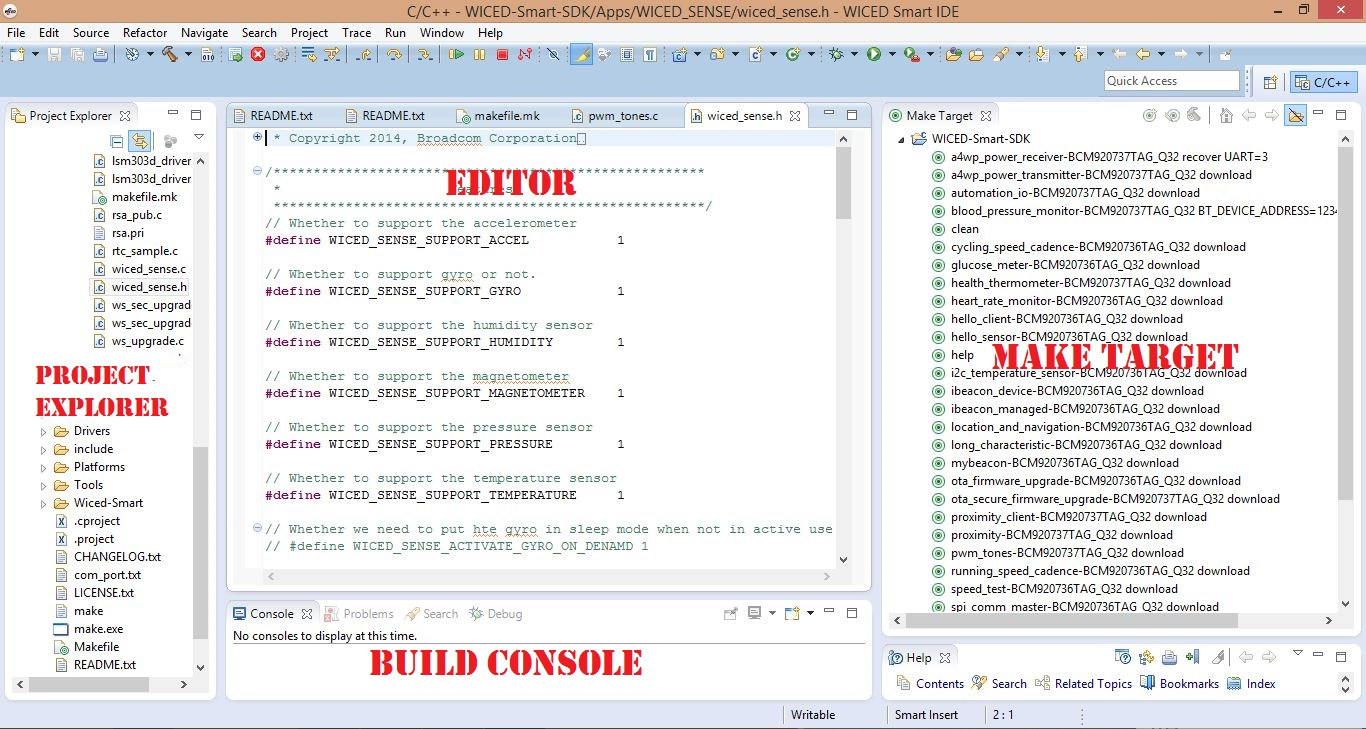
\includegraphics[scale=0.4]{Wiced-sdk.JPG}
	\end{figure}
	
	\item Project Explorer - This section provides list of all the projects that have been created.It contains all the c , h and makefile requird to build the project.
	\item Editor - This window provides space to write the code according to our project. The code is written in C language.
	\item Make Target - It creates a target for your device. When you click on the specified target, that code begins to compile and is flashed to your device.
	\item Build Console - It shows the current status while compiling and flashing the code to the device.
\end{itemize}

\newpage
\section{Creating a new project}
 \begin{itemize}
 \item Download the project from the link given
\href{https://community.cypress.com/docs/DOC-2213}{here}
 
 
  \begin{figure}[h]
    \centering
	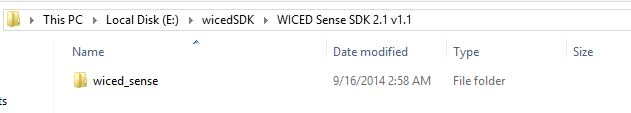
\includegraphics[scale=0.6]{download.JPG}
	\end{figure}
 \end{itemize} 
 
  \begin{itemize}
 \item Copy the project to the apps directory of wiced sense.
 \item Open > New > Folder.
 \begin{figure}[h]
    \centering
	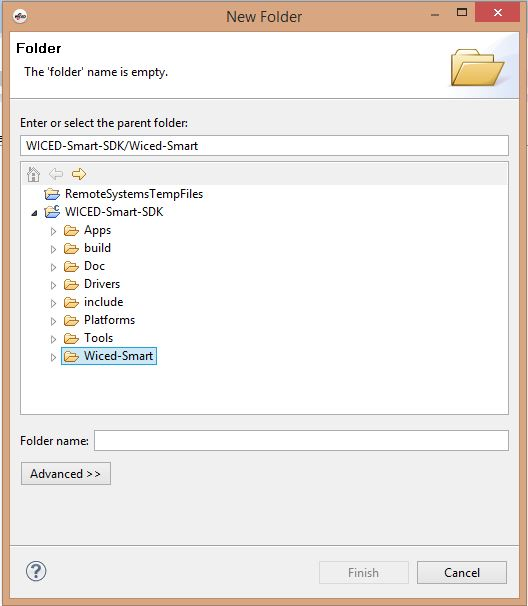
\includegraphics[scale=0.4]{newproj.JPG}
	\end{figure}
 \item Insert the name of parent folder to the path where you have placed the wiced sense in apps. 

	 \begin{figure}[h]
    \centering
	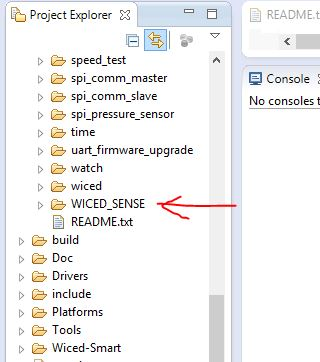
\includegraphics[scale=0.6]{wiced.JPG} 
	\end{figure}
	
	\item When you click OK you will see a project named Wiced Sense created in project explorer section
		
    \newpage
	 \begin{figure}[h]
    \centering
	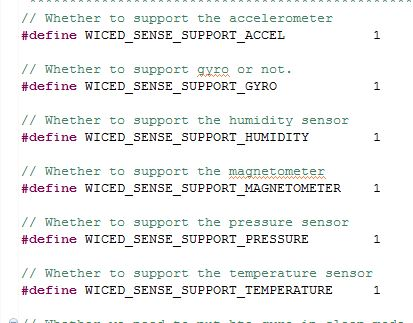
\includegraphics[scale=0.6]{support.JPG}
	\end{figure}
	\item Now you can Set the sensor to be ON/OFF by making the bit in the above code ON or OFF.
	
	 \begin{figure}[h]
    \centering
	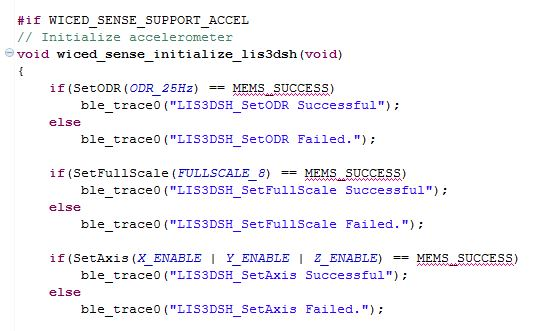
\includegraphics[scale=0.6]{wiced_accel.JPG}
	\end{figure}
	
	\item We can set the refresh rate to take the sensor data at particular interval. Now it is set to 25Hz as ODR register is set to 25Hz.
	\item We can set the full scale range of a particular sensor. Right Now it is set to 8g. It can be changed to 2g,4g,8g,16g.

	\item We can also make the particular axis of the sensors ON/Off. 
	
	\item Now the value from this function is sent to the driver code of that sensor.
	
	\newpage
	
	\item Control register to set the fullscale.
	 
	\begin{figure}[h]
    \centering
	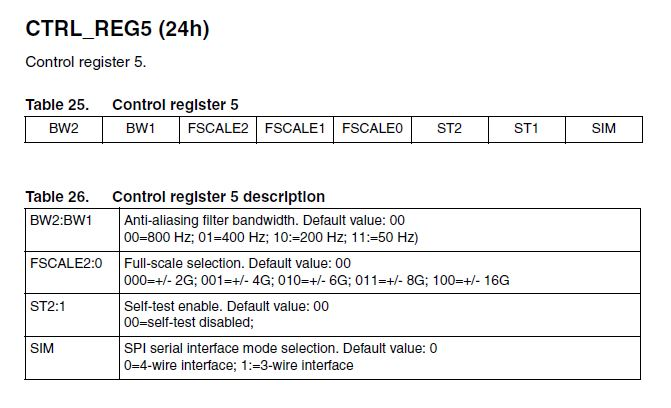
\includegraphics[scale=0.6]{setting_range1.JPG}
	\end{figure}
	
	\item 100 is passed through value variable which sets the fullscale range to 8g.
	
	 \begin{figure}[h]
    \centering
	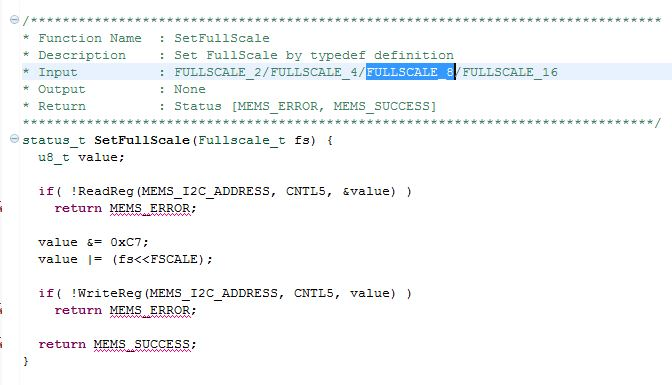
\includegraphics[scale=0.6]{setting_range0.JPG}
	\end{figure}
	
	

	\newpage
	
	\item Now we will make a new target file which will enable us to flash the code.
	\begin{figure}[h]
    \centering
	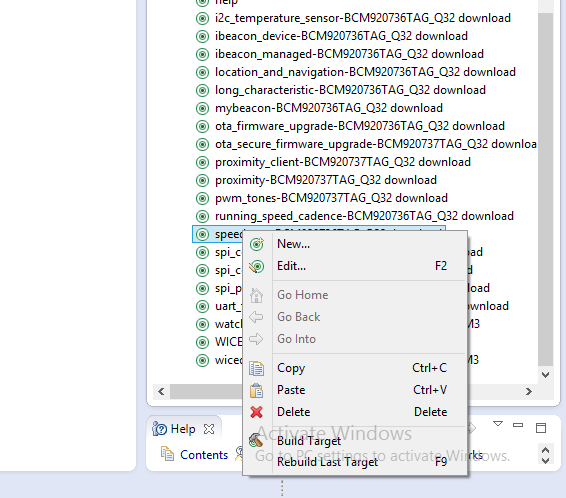
\includegraphics[scale=0.6]{newtarget.png}
	\end{figure}
	
		\item Give the name of the target file same as that in apps section i.e {WICED-SENSE-BCM920737TAG-Q32} download for me.
		\begin{figure}[h]
    \centering
	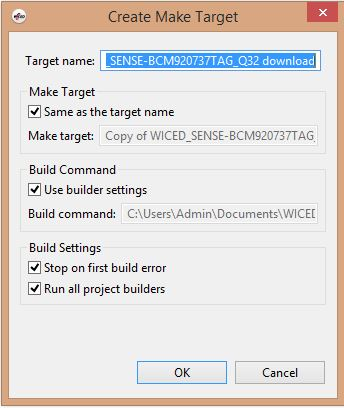
\includegraphics[scale=0.6]{createmaketarget.JPG}
	\end{figure}
	

	\item Double click the created target file and it will start compiling the code.
	\item Current process can be observed in console.
	\item You will get Application Running at the end, it means that you have flashed the code successfully.
	
	\newpage
	\section{Reference}
	
	https://community.cypress.com/docs/DOC-1759 \\
	https://community.cypress.com/docs/DOC-1766
	
	
	
	
	
	
	
	
	
	
	
	
	
	
	
	
	
	
	
 \end{document}